\documentclass[12pt,twoside]{article}

\usepackage[dvipsnames]{xcolor}
\usepackage{tikz,graphicx,amsmath,amsfonts,amscd,amssymb,bm,cite,epsfig,epsf,url}
\usepackage[hang,flushmargin]{footmisc}
\usepackage[colorlinks=true,urlcolor=blue,citecolor=blue]{hyperref}
\usepackage{amsthm,multirow,wasysym,appendix}
\usepackage{array,subcaption} 
%
% \usepackage[small,bf]{caption}
\usepackage{bbm}
\usepackage{pgfplots}
\usetikzlibrary{spy}
\usepgfplotslibrary{external}
\usepgfplotslibrary{fillbetween}
\usetikzlibrary{arrows,automata}
\usepackage{thmtools}
\usepackage{blkarray} 
\usepackage{textcomp}
\usepackage[left=0.8in,right=1.0in,top=1.0in,bottom=1.0in]{geometry}
\usepackage{pifont}
\usepackage{tikz-qtree}

%% Probability operators and functions
%
% \def \P{\mathrm{P}}
\def \P{\mathrm{P}}
\def \E{\mathrm{E}}
\def \Var{\mathrm{Var}}
\let\var\Var
\def \Cov {\mathrm{Cov}} \let\cov\Cov
\def \MSE {\mathrm{MSE}} \let\mse\MSE
\def \sgn {\mathrm{sgn}}
\def \R {\mathbb{R}}
\def \C {\mathbb{C}}
\def \N {\mathbb{N}}
\def \Z {\mathbb{Z}}
\def \cV {\mathcal{V}}
\def \cS {\mathcal{S}}

\newcommand{\RR}{\ensuremath{\mathbb{R}}}

\DeclareMathOperator*{\argmin}{arg\,min}
\DeclareMathOperator*{\argmax}{arg\,max}
\newcommand{\red}[1]{\textcolor{red}{#1}}
\newcommand{\blue}[1]{\textcolor{blue}{#1}}
\newcommand{\green}[1]{\textcolor{ForestGreen}{ #1}}
\newcommand{\fuchsia}[1]{\textcolor{RoyalPurple}{ #1}}



%
%% Probability distributions
%
%\def \Bern    {\mathrm{Bern}}
%\def \Binom   {\mathrm{Binom}}
%\def \Exp     {\mathrm{Exp}}
%\def \Geom    {\mathrm{Geom}}
% \def \Norm    {\mathcal{N}}
%\def \Poisson {\mathrm{Poisson}}
%\def \Unif    {\mathrm {U}}
%
\DeclareMathOperator{\Norm}{\mathcal{N}}

\newcommand{\bdb}[1]{\textcolor{red}{#1}}

\newcommand{\ml}[1]{\mathcal{ #1 } }
\newcommand{\wh}[1]{\widehat{ #1 } }
\newcommand{\wt}[1]{\widetilde{ #1 } }
\newcommand{\conj}[1]{\overline{ #1 } }
\newcommand{\rnd}[1]{\tilde{ #1 } }
\newcommand{\rv}[1]{ \rnd{ #1}  }
\newcommand{\rM}{\rnd{ m}  }
\newcommand{\rx}{\rnd{ x}  }
\newcommand{\ry}{\rnd{ y}  }
\newcommand{\rz}{\rnd{ z}  }
\newcommand{\ra}{\rnd{ a}  }
\newcommand{\rb}{\rnd{ b}  }
\newcommand{\rt}{\rnd{ t}  }
\newcommand{\rs}{\rnd{ s}  }


\newcommand{\rpc}{\widetilde{ pc}  }
\newcommand{\rndvec}[1]{\vec{\rnd{#1}}}

\def \cnd {\, | \,}
\def \Id { I }
\def \J {\mathbf{1}\mathbf{1}^T}

\newcommand{\op}[1]{\operatorname{#1}}
\newcommand{\setdef}[2]{ := \keys{ #1 \; | \; #2 } }
\newcommand{\set}[2]{ \keys{ #1 \; | \; #2 } }
\newcommand{\sign}[1]{\op{sign}\left( #1 \right) }
\newcommand{\trace}[1]{\op{tr}\left( #1 \right) }
\newcommand{\tr}[1]{\op{tr}\left( #1 \right) }
\newcommand{\inv}[1]{\left( #1 \right)^{-1} }
\newcommand{\abs}[1]{\left| #1 \right|}
\newcommand{\sabs}[1]{| #1 |}
\newcommand{\keys}[1]{\left\{ #1 \right\}}
\newcommand{\sqbr}[1]{\left[ #1 \right]}
\newcommand{\sbrac}[1]{ ( #1 ) }
\newcommand{\brac}[1]{\left( #1 \right) }
\newcommand{\bbrac}[1]{\big( #1 \big) }
\newcommand{\Bbrac}[1]{\Big( #1 \Big)}
\newcommand{\BBbrac}[1]{\BIG( #1 \Big)}
\newcommand{\MAT}[1]{\begin{bmatrix} #1 \end{bmatrix}}
\newcommand{\sMAT}[1]{\left(\begin{smallmatrix} #1 \end{smallmatrix}\right)}
\newcommand{\sMATn}[1]{\begin{smallmatrix} #1 \end{smallmatrix}}
\newcommand{\PROD}[2]{\left \langle #1, #2\right \rangle}
\newcommand{\PRODs}[2]{\langle #1, #2 \rangle}
\newcommand{\der}[2]{\frac{\text{d}#2}{\text{d}#1}}
\newcommand{\pder}[2]{\frac{\partial#2}{\partial#1}}
\newcommand{\derTwo}[2]{\frac{\text{d}^2#2}{\text{d}#1^2}}
\newcommand{\ceil}[1]{\lceil #1 \rceil}
\newcommand{\Imag}[1]{\op{Im}\brac{ #1 }}
\newcommand{\Real}[1]{\op{Re}\brac{ #1 }}
\newcommand{\norm}[1]{\left|\left| #1 \right|\right| }
\newcommand{\norms}[1]{ \| #1 \|  }
\newcommand{\normProd}[1]{\left|\left| #1 \right|\right| _{\PROD{\cdot}{\cdot}} }
\newcommand{\normTwo}[1]{\left|\left| #1 \right|\right| _{2} }
\newcommand{\normTwos}[1]{ \| #1  \| _{2} }
\newcommand{\normZero}[1]{\left|\left| #1 \right|\right| _{0} }
\newcommand{\normTV}[1]{\left|\left| #1 \right|\right|  _{ \op{TV}  } }% _{\op{c} \ell_1} }
\newcommand{\normOne}[1]{\left|\left| #1 \right|\right| _{1} }
\newcommand{\normOnes}[1]{\| #1 \| _{1} }
\newcommand{\normOneTwo}[1]{\left|\left| #1 \right|\right| _{1,2} }
\newcommand{\normF}[1]{\left|\left| #1 \right|\right| _{\op{F}} }
\newcommand{\normLTwo}[1]{\left|\left| #1 \right|\right| _{\ml{L}_2} }
\newcommand{\normNuc}[1]{\left|\left| #1 \right|\right| _{\ast} }
\newcommand{\normOp}[1]{\left|\left| #1 \right|\right|  }
\newcommand{\normInf}[1]{\left|\left| #1 \right|\right| _{\infty}  }
\newcommand{\proj}[1]{\mathcal{P}_{#1} \, }
\newcommand{\diff}[1]{ \, \text{d}#1 }
\newcommand{\vc}[1]{\boldsymbol{\vec{#1}}}
\newcommand{\rc}[1]{\boldsymbol{#1}}
\newcommand{\vx}{\vec{x}}
\newcommand{\vy}{\vec{y}}
\newcommand{\vz}{\vec{z}}
\newcommand{\vu}{\vec{u}}
\newcommand{\vv}{\vec{v}}
\newcommand{\vb}{\vec{\beta}}
\newcommand{\va}{\vec{\alpha}}
\newcommand{\vaa}{\vec{a}}
\newcommand{\vbb}{\vec{b}}
\newcommand{\vg}{\vec{g}}
\newcommand{\vw}{\vec{w}}
\newcommand{\vh}{\vec{h}}
\newcommand{\vbeta}{\vec{\beta}}
\newcommand{\valpha}{\vec{\alpha}}
\newcommand{\vgamma}{\vec{\gamma}}
\newcommand{\veta}{\vec{\eta}}
\newcommand{\vnu}{\vec{\nu}}
\newcommand{\rw}{\rnd{w}}
\newcommand{\rvnu}{\vc{\nu}}
\newcommand{\rvv}{\rndvec{v}}
\newcommand{\rvw}{\rndvec{w}}
\newcommand{\rvx}{\rndvec{x}}
\newcommand{\rvy}{\rndvec{y}}
\newcommand{\rvz}{\rndvec{z}}
\newcommand{\rvX}{\rndvec{X}}


\newtheorem{theorem}{Theorem}[section]
% \declaretheorem[style=plain,qed=$\square$]{theorem}
\newtheorem{corollary}[theorem]{Corollary}
\newtheorem{definition}[theorem]{Definition}
\newtheorem{lemma}[theorem]{Lemma}
\newtheorem{remark}[theorem]{Remark}
\newtheorem{algorithm}[theorem]{Algorithm}

% \theoremstyle{definition}
%\newtheorem{example}[proof]{Example}
\declaretheorem[style=definition,qed=$\triangle$,sibling=definition]{example}
\declaretheorem[style=definition,qed=$\bigcirc$,sibling=definition]{application}

%
%% Typographic tweaks and miscellaneous
%\newcommand{\sfrac}[2]{\mbox{\small$\displaystyle\frac{#1}{#2}$}}
%\newcommand{\suchthat}{\kern0.1em{:}\kern0.3em}
%\newcommand{\qqquad}{\kern3em}
%\newcommand{\cond}{\,|\,}
%\def\Matlab{\textsc{Matlab}}
%\newcommand{\displayskip}[1]{\abovedisplayskip #1\belowdisplayskip #1}
%\newcommand{\term}[1]{\emph{#1}}
%\renewcommand{\implies}{\;\Rightarrow\;}



\begin{document}

\begin{center}
{\large{\textbf{Homework 7}} } \vspace{0.2cm}\\
Due Mar 26 at 11 pm
\\
\end{center}
Unless stated otherwise, justify any answers you give.
You can work in groups, but each
student must write their own solution based on their own
understanding of the problem.

When uploading your homework to Gradescope you will have to
select the relevant pages for each question.  Please submit each
problem on a separate page (i.e., 1a and~1b can be on the same page but 1
and 2 must be on different pages).  We understand that this may be
cumbersome but this is the best way for the grading team to grade your
homework assignments and provide feedback in a timely manner.  Failure
to adhere to these guidelines may result in a loss of points.
Note that it may take some time to
select the pages for your submission.  Please plan accordingly.  We
suggest uploading your assignment at least 30 minutes before the deadline
so you will have ample time to select the correct pages for your
submission.  If you are using \LaTeX, consider using the minted or
listings packages for typesetting code.  
\\

\begin{enumerate}

\item (Sign test) The sign test is a nonparametric two-sample test. Given $n$ pairs of data $(x_1,y_1)$, $(x_2,y_2)$, \ldots, $(x_n,y_n)$, the null hypothesis is that the first and second entries of each pair belong to the same distribution. The test statistic is
\begin{align}
t & = \sum_{i=1}^{n} 1\brac{y_i > x_i},
\end{align}
where $1\brac{y_i > x_i}$ is an indicator function that is equal to 1 if $y_i > x_i$ and 0 otherwise.  
\begin{enumerate}
\item If $\ra$ and $\rb$ are independent continuous random variables with the same distribution, what is the probability that $\ra > \rb$?
\begin{itemize}
  \color{blue}
  \item $P(\Tilde{a}\geq \Tilde{b})=\int_{b\in \mathbb{R}}P(\Tilde{a}\in[b,\infty],\Tilde{b}\in[-\infty,b])
  db=\int_{b\in \mathbb{R}}P(\Tilde{a}\in[b,\infty])P(\Tilde{b}\in[-\infty,b])
  db=\int_{b\in \mathbb{R}}(1-F_{\Tilde{a}}(b))F_{\Tilde{b}}(b)
  db=\int_{b\in \mathbb{R}}(1-F_{\Tilde{b}}(b))F_{\Tilde{b}}(b)
  db=\frac{1}{2}$
\end{itemize}

\item Derive the distribution of the test statistic of the sign test under the null hypothesis that the data are independent samples from the same continuous distribution.
\begin{itemize}
  \color{blue}
  \item consider a random varible $\Tilde{t_i}=1(\Tilde{y}_i\geq \Tilde{x}_i)$ we can think of $\Tilde{t}_i$ as a bernoulli random variable with parameter $\theta$
  \item thus we can think of our test stat under the null as the sum of independent identically distributed bernoulli random variables and thus distributed as a binomial with parameters n, $\theta_{null}$ 
  \item where  $\theta_{null}$ represents the $P(x_i\geq y_i)$, which under the null being $\Tilde{x}, \Tilde{y}$ are distributed the same, we would have $\theta_{null}=0.5$
  \item thus we know that the test stat under the null is distributed as a binomial with parameter n, .5 that is $t\sim b(n,0.5)$
\end{itemize}

\item Your friend is convinced that in general the left ear of most people is longer than the right ear. You measure the ears of some of your other friends and obtain the following data (in inches).
\renewcommand{\arraystretch}{1.5}
\begin{center}
\begin{tabular}{ | c | c | c | c | c | c | c | c | c | c | c |  } % c | c | c l c | c | c | c | c | c | }
  \hline			
Left  & 2.4 & 2.7 & 3.2 & 2.3 & 2.0 & 2.6 & 3.2 & 2.3 & 2.9 & 2.3  \\
  \hline			
 Right  &  2.2 & 2.6 & 3.3 & 2.2 & 2.1 & 2.5 & 3.1 & 2.5 & 2.7 & 2.2  \\
  \hline  
 \end{tabular}
\end{center} 
Apply the sign test to compute a p value associated to the null hypothesis that the left and right ear have the same length. 
\begin{itemize}
  \color{blue}
  \item we know our p-value is $P(t\leq \Tilde{t}_{null})=(1-F_{\Tilde{t}_{null}}(t))=\Sigma_{i=t}^{10}\begin{pmatrix}
    10\\i
  \end{pmatrix}(0.5)^{i}(0.5)^{10-i}=\Sigma_{i=t}^{10}\begin{pmatrix}
    10\\i
  \end{pmatrix}(0.5)^{10}$
  \item we can see in our data $n=10$ as there are 10 samples and $k=7$ as in 7 cases the left ear length is greater than the right ear length
  \item so computing this out we see that our p value ends up being 0.171875
\end{itemize}

\item Is the sign test still valid for the null hypothesis that each pair of data $(x_i,y_i)$ are sampled from the same continuous distribution, but these distributions are different for different values of $i$?   
\begin{itemize}
  \color{blue}
  \item yes it should still hold
  \item at each sample we are finding $P(y_i\geq x_i)$
  \item and regardless of how $\Tilde{y}_i,\tilde{x}_i$ are distributed under the null hypothesis we assume they have the same distribution thus, $P(y_i\geq x_i)=0.5$ 
  \item the above implies that regardless of the actual distribution  $\Tilde{y}_i,\tilde{x}_i$ we know $1(\tilde{x}_i\geq \Tilde{y}_i)=\tilde{t}_i\sim \text{bernoulli}(0.5)$
  \item which implies $\Sigma_{1=1}^{n}1(\Tilde{y}_i\geq \tilde{x}_i)=\Sigma_{1=1}^{n}\tilde{t}_i=\tilde{t}\sim b(n,0.5)$
  \item and thus the sign test would still hold. 
\end{itemize}
\newpage
\end{enumerate}

\item (Drug design) 
A company wants to design a drug to extend the life of patients with a certain disease. From past data, the survival time of the patients is known to be exponential with parameter 1. The company has a large number of promising drug candidates. When a candidate is effective, it modifies the survival time to be exponential with parameter $\theta$. Otherwise it does not affect the survival time at all. In order to evaluate the candidates, each one is given to a different patient. A hypothesis test is then applied where the test statistic is the survival time of the patient. The null hypothesis is that the drug does not work and therefore the survival time is exponential with parameter 1. 

\begin{enumerate}
\item Derive the pdf of the p value when the drug is effective as a function of $\theta$. Plot it for $\theta$ equal to 1 and to 0.1.
\begin{itemize}
  \color{blue}
  \item call $H_{0}$ the null hypothesis and $H_{1}$ the alternative hypothesis
  \item given we know the alternative hypothesis is true we can write the p value as $pv(t)=P(\tilde{t}\geq t|H_0)=P(\tilde{t}\geq t|H_1)=e^{-\theta t}\sim e(\theta)$
  \item so our pdf is $\theta e^{-\theta t}$
  \item 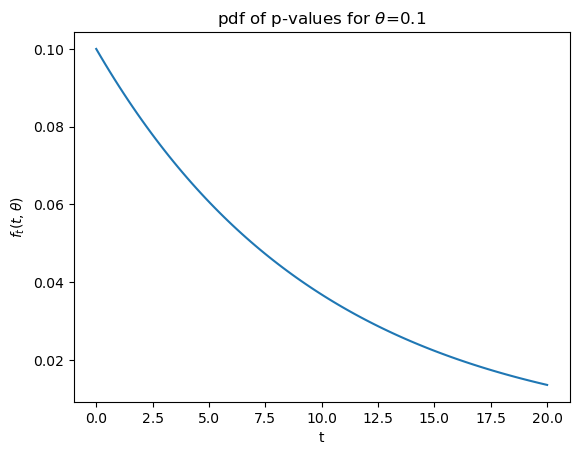
\includegraphics{/home/buzgalbraith/work/school/spring_2023/probaility-theroy-2-2023/homework/homework_7/immages/2a_1.png}
  \item 
  \item 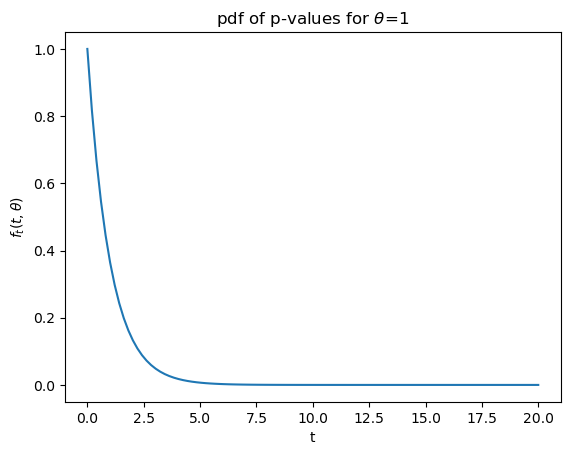
\includegraphics{/home/buzgalbraith/work/school/spring_2023/probaility-theroy-2-2023/homework/homework_7/immages/2a_2.png}
\end{itemize}

\item Derive the pdf of the p value if the probability that the drug is effective is 1/20 (i.e. only 5\% of the candidates are effective) as a function of $\theta$. Plot the pdf for $\theta:=0.1$. 
\begin{itemize}
  \color{blue}
  \item by the law of total probability $pv(t)=P(\tilde{t}_{null}\geq t)=P(\tilde{t}_{null}\geq t|H_0)P(H_0)+P(\tilde{t}_{null}\geq t|H_1)P(H_1)$
  \item then using what we derived in last question and the information in this question we can write $pv(t)=P(\tilde{t}_{null}\geq t)=\frac{19}{20}(1-F_{\tilde{t}_{null}}(t))+\frac{1}{20}(1-F_{\tilde{t}_{\theta}}(t))=\frac{19}{20}(e^{-t})+\frac{1}{20}(e^{-\theta t})$
  \item then as we know difertiation is linear the pdf is just the sum of there darivatives with respect to $\theta$ that is $f_{pv(t)}=e^{-t}+\theta e^{-\theta t}$
  \item 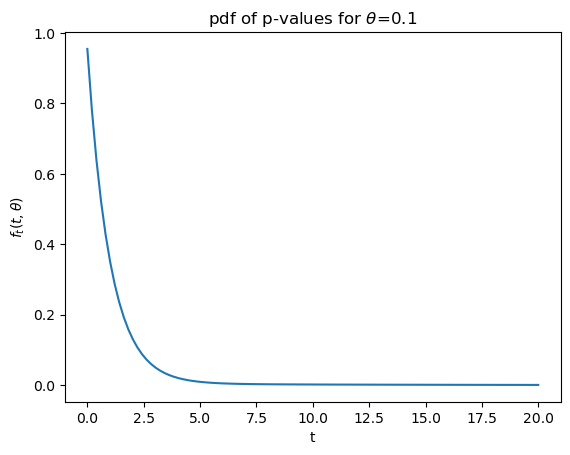
\includegraphics{/home/buzgalbraith/work/school/spring_2023/probaility-theroy-2-2023/homework/homework_7/immages/2b_1.png} 
\end{itemize}

\item If we reject the null hypothesis, what is the conditional probability that there is a false positive and the drug candidate doesn't actually work? Derive the conditional probability as a function of the significance level $\alpha$ and of $\theta$, and report it for $\alpha = 0.05$ and $\theta:=0.1$. 
\begin{itemize}
  \color{blue}
  \item first we need to solve for $t_{thresh}$ under the null hypothiss such that $t_{thresh}:=argmin_{t}\{ t:pv(t)\leq \alpha | H_{0}\}=argmin_{t}\{ t:P(\Tilde{t}\geq t)\leq \alpha | H_{0}\}
  =argmin_{t}\{t:1-F_{\tilde{t}_{null}}(t)\leq \alpha\}=argmin_{t}\{t:e^{-(t)}\leq \alpha\}=-ln(\alpha)$
  \item so if we reject the null we know that $\Tilde{t}\leq t_{thresh}$
  \item given this is the case our likelihood of a false positive is thus $P(H_{0}|\tilde{t}\leq t_{thresh})$ that is the likelihood the null is true given we reject the null 
  \item we can write this with bayes therome as  $P(H_{0}|\tilde{t}\leq t_{thresh})=\frac{P(H_{0},\tilde{t}\leq t_{thresh})}{P(\tilde{t}\leq t_{thresh})}$
  \item so first we know $P(H_0, \tilde{t}\leq t_{thresh})$ is the case where the null is true but we reject the null that is we have a false postive is $P(H_0)\alpha$
  \item now consider $P(\tilde{t}\leq t_{thresh})=P(\tilde{t}\leq t_{thresh}|H_0)P(H_0)+P(\tilde{t}\leq t_{thresh}|H_1)P(H_1)=\alpha(P(H_0))+(1-F_{\theta}(t_{threshold}))(1-P(H_0))$
  \item so this equals $\frac{P(H_0)\alpha}{\alpha P(H_0)  +(1-F_{\theta_t}(t_{threshold}))(1-P(H_0)) }=\frac{P(h_0)\alpha
  }{P(h_0)\alpha + P(h_a)(e^{-\theta ln(\alpha)})}$  
  \item i am going to assume that we are supposed to use $P(H_1)=\frac{1}{2}$ since there is no other indication of what value to use 
  \item doing this out i got 0.04627870362231976 as the liklyhood of the null being true  given we rejet the null
  \item that is encouragaing since the value is around 5\% which is where we expect it to be. 
\end{itemize}


\item Derive the conditional probability that the drug candidate doesn't work given that the p value equals $\pi$, as a function of $\pi$ and $\theta$. Plot the function for $0 \leq \pi \leq 0.05$ and $\theta := 0.1$. Based on your result, suggest a strategy to select candidates sequentially for follow-up testing.
\begin{itemize}
  \color{blue}
  \item so we are looking for $P(H_0|pv(t)=\pi)=\frac{P(Pv(t)=\pi|H_0)P(H_0)}{P(Pv(t)=\pi|H_0)P(H_0)+P(Pv(t)=\pi|H_1P(H_1)}
  =\frac{e^{-\pi }P(H_0)}{e^{-\pi t}P(H_0)+e^{-\theta \pi }P(H_1)} 
  $
  \item again we are not explicitly given a value for the likelihood of each hypothesis i am going to assume $P(H_0)=P(H_1)$ since i guess that makes the least assumptions?
  \item 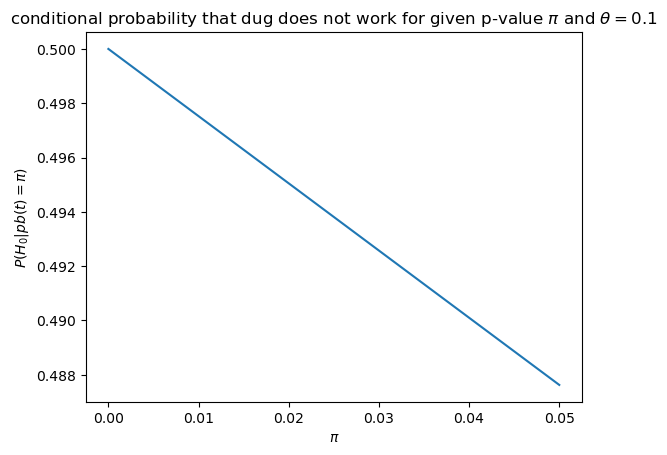
\includegraphics{/home/buzgalbraith/work/school/spring_2023/probaility-theroy-2-2023/homework/homework_7/immages/2c_1.png} 
\end{itemize}

\end{enumerate}
\newpage
\item (P-hacking) 
\begin{enumerate}
\item If $\rnd{u}$ is a uniform random variable between 0 and 1, derive the conditional pdf of $\rnd{u}$ conditioned on the event $\rnd{u}\leq \alpha$ for $0 <\alpha < 1$. 
\begin{itemize}
  \color{blue}
  \item consider an arbitrary value k, $P(\Tilde{u}\leq k|\tilde{u}\leq \alpha)$
\item we can see that $1=\int_{k\in \mathbb{R}}f_{\tilde{u}\leq \alpha}(k)dk=\int_{k\in \mathbb{-\infty}}^{\alpha}f_{\tilde{u}\leq \alpha}(k)+\int_{0}^{\alpha}f_{\tilde{u}\leq \alpha}(k)+\int_{\alpha}^{\infty}f_{\tilde{u}\leq \alpha}(k)dk=\int_{0}^{\alpha}f_{\tilde{u}\leq \alpha}(k)dk=(1-\alpha)f_{\tilde{u}\leq \alpha}=1\Rightarrow f_{\tilde{u}\leq \alpha}=\frac{1}{\alpha}$ 
\end{itemize}

\item The histogram of the p values in the publications of a research group looks like this:
\begin{center}
 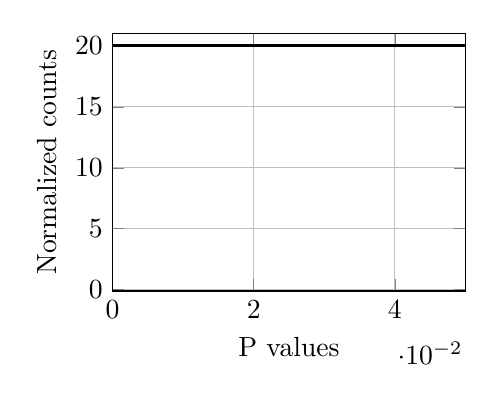
\begin{tikzpicture}% [font=\footnotesize]
\begin{axis}[xmin= 0, xmax=0.05, ymin=-0.1, ymax=21, xlabel=P values,
ylabel=Normalized counts,grid,%extra x ticks={0.5, 2.5},
width=0.5\textwidth,
        height=0.4\textwidth]
\addplot[black,very thick, domain=0:0.05, samples=3] {20};
\end{axis}
\end{tikzpicture}
\end{center}
What does this suggest? 
\begin{itemize}
  \color{blue}
  \item this suggest the group is not p-hacking as there is a uniform distribution over the interval as we would expect to see. 
\end{itemize}

\item If the total number of p values is 100, estimate the number of results that the research group has not published. 
\begin{itemize}
  \color{blue}
  \item assuming a uniform distribution of p values we would expect for there to be k total studies where k is  $k:\frac{5}{100}*k=100\Rightarrow k=2,000$
  \item thus the number of unpublished studies would be 1,900
\end{itemize}

\end{enumerate}
\newpage
\item (Airbnb Pricing)
Airbnb prices oftern vary by neighborhood. In this problem, our conjecture is that prices in the Upper East Side and Upper West Side are different. Our goal is to evaluate this conjecture using hypothesis testing. The null hypothesis is that the price distribution is the same. Based on the \textit{price} and \textit{neighbourhood} columns in the open Airbnb dataset in \texttt{AB\_NYC\_2019.csv}, we conduct parametric and non-parametric hypothesis testing. 
\begin{enumerate} 

\item Assuming the price in the two neighbourhoods are two Gaussian random variables with known population standard deviation $240.15$, apply a parametric two-sample test. Select a test statistic and compute the p-value.
\begin{itemize}
  \color{blue}
  \item let people in the upper east side be group a and poeple in the upper west side be group b 
  \item and let $x_i$ be a random varible representing the price of data point i's Airbnb
  \item let the test stat be $t=|\frac{1}{n_{a}}\Sigma_{i\in a}x_i-\frac{1}{n_{b}}\Sigma_{i\in b}x_i|$
  \item i am doing a two sample test, as in our conjecture we do not specficy that one neighborhood is more expensive than the other
  \item doing this we get a p value of 0.0522
\end{itemize}

\item Plot the histograms of prices in the two neighbourhoods. What do you think might be problematic about the test statistic you selected for the parametric test? 
\begin{itemize}
  \color{blue}
  \item 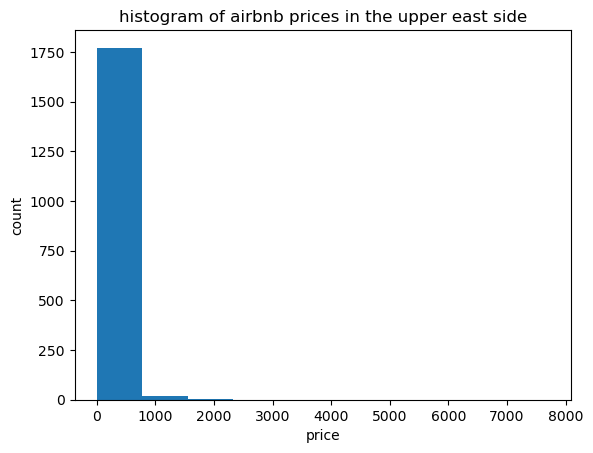
\includegraphics{/home/buzgalbraith/work/school/spring_2023/probaility-theroy-2-2023/homework/homework_7/immages/4b_1.png} 
   \item 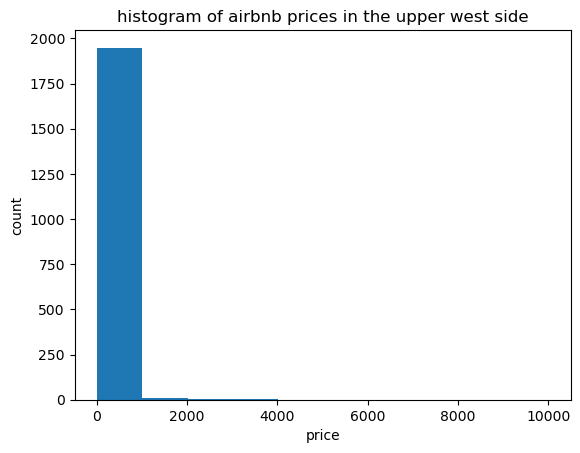
\includegraphics{/home/buzgalbraith/work/school/spring_2023/probaility-theroy-2-2023/homework/homework_7/immages/4b_2.png}  
  \item as can be seen from this graph both are clearly not gaussian, and infact are heavily sckewed by there outliers
\end{itemize}

\item Select another test statistic that is more robust to outliers. Apply a permutation test and compute the corresponding p-value.
\begin{itemize}
  \color{blue}
  \item let people in the upper east side be group a and poeple in the upper west side be group b 
  \item and let $x_i$ be a random varible representing the price of data point i's Airbnb
  \item let the test stat be $t=|\text{median(group a)}-\text{median(group b)}|$
  \item running this for 1000 monte carlo simultions of permutations in the multiset i found a p-value of 0.926
 
\end{itemize}

\end{enumerate}
\end{enumerate}
\end{document}
